\subsubsection{Generatore trascrizioni e Generatore audio}

\begin{scenario}{Scenario: Trascrizione di appunti audio tramite Sbobinatore AI}
  Ho deciso di provare lo strumento chiamato \textit{«Sbobinatore AI»} su
  BrainBox per convertire la registrazione audio di una lezione in testo. Già dal nome, in realtà, \textbf{non mi è del tutto chiara l'esatta funzione dello strumento} e cosa farà di preciso, ma decido comunque di procedere. Accedo alla sezione dedicata con l'obiettivo di caricare il mio file e lasciare che l'intelligenza artificiale esegua la trascrizione.

  Osservando la pagina vuota, cerco d'istinto un pulsante di caricamento al centro dello schermo. Noto una scritta che dice \textit{«Inizia caricando il tuo primo file!»}, ma \textbf{non avendo l'aspetto di un pulsante cliccabile}, la ignoro. Solo dopo aver guardato meglio la pagina, mi accorgo che il pulsante per creare una nuova trascrizione si trova in alto, nella barra di intestazione: una \textbf{posizione poco
  intuitiva} rispetto a dove stavo guardando.

  Una volta cliccato il pulsante, si apre la schermata per il caricamento. Mi viene chiesto di inserire diverse informazioni.
  Mentre mi preparo a caricare il file, mi rendo conto che \textbf{non è specificato da nessuna parte} quali siano i formati audio accettati né se ci sia un limite di grandezza per il documento. Compilo il campo obbligatorio per il nome e avvio l'operazione.

  A questo punto, il caricamento fallisce e compare un \textbf{messaggio di errore in lingua inglese}. L'avviso è \textbf{molto generico} e non mi spiega il motivo del problema: non so se ho sbagliato il formato o se il file era troppo grande. Questo mi lascia incerto su come rimediare all'errore, oltre a risultare fuori posto in una pagina che finora era tutta in italiano.

  Risolto il problema per tentativi, riesco finalmente ad avviare l'elaborazione. Tuttavia, noto che \textbf{lo strumento non fornisce alcuna indicazione chiara} su come stia procedendo il lavoro. Senza un \textbf{indicatore visivo di avanzamento} o una stima del tempo necessario, resto ad attendere senza sapere se il sistema stia
  effettivamente lavorando o se si sia bloccato.

  Quando il testo finalmente compare, noto che la trascrizione si presenta come \textbf{un unico e lungo blocco di testo}, senza alcuna suddivisione in paragrafi o pause che ne facilitino la lettura.

  Infine, scopro che \textbf{non c'è un comando per salvare il testo} direttamente tra i miei appunti sulla piattaforma: per poterlo conservare e correggere, devo prima scaricare il documento sul mio
  computer, apportare le modifiche e poi ricaricare il file manualmente nella sezione principale dei miei appunti.
\end{scenario}

Lo scenario di utilizzo dello Sbobinatore AI ha evidenziato alcune delle criticità più significative dell'intera applicazione. L'utente si trovava davanti a una pagina dedicata con un nome poco chiaro, pulsanti di avvio in posizioni non intuitive, nessuna indicazione sui formati accettati o sui limiti di dimensione, messaggi di errore in inglese e generici, nessun feedback visivo durante l'elaborazione, output non strutturato e, soprattutto, nessuna possibilità di salvare il risultato direttamente tra i propri appunti senza dover scaricare, modificare e ricaricare 
manualmente il file. Quest'ultima criticità rappresentava il problema di usabilità più grave dell'intera sezione, in quanto interrompeva completamente il flusso di lavoro dell'utente e vanificava l'utilità pratica dello strumento.

La scelta progettuale più rilevante adottata per risolvere questi problemi è stata quella di eliminare le pagine dedicate agli strumenti AI e di integrare le funzionalità di generazione direttamente nella sezione \textit{Appunti}. Questa decisione ha permesso di risolvere in modo strutturale il problema del salvataggio: i file generati, trascrizioni e audio note, vengono ora creati e archiviati direttamente nella sezione \textit{Appunti}, dove l'utente può organizzarli insieme agli altri materiali di studio, allegarli agli esami e gestirli liberamente senza passaggi intermedi. Centralizzare tutto in un unico spazio ha inoltre eliminato la frammentazione tra sezioni separate che rendeva difficile orientarsi 
nell'applicazione.

\paragraph{Design pattern applicati}
\begin{itemize}
\item \textbf{Input Hints} (Tidwell): Il pattern suggerisce di fornire spiegazioni, vincoli o suggerimenti contestuali vicino ai campi di input per prevenire errori prima che accadano. Questo è fondamentale per gestire le aspettative dell'utente riguardo a limiti tecnologici o formati supportati. Nella versione precedente lo strumento non indicava i formati audio accettati né gli eventuali limiti di dimensione, costringendo l'utente a procedere per tentativi; nella versione riprogettata questi vincoli sono resi espliciti direttamente nel primo step di caricamento.

Problemi di usabilità risolti:
\begin{itemize}
  \item P70 (Mancanza di spiegazione sui limiti tecnologici): Nel primo step del caricamento sono stati esplicitati i formati audio supportati e, tramite un'avvertenza dedicata, è stato chiarito che gli strumenti AI possono commettere errori di precisione.
\end{itemize}

\begin{figure}[H]
    \centering
    \begin{subfigure}[b]{0.47\textwidth}
        \centering
        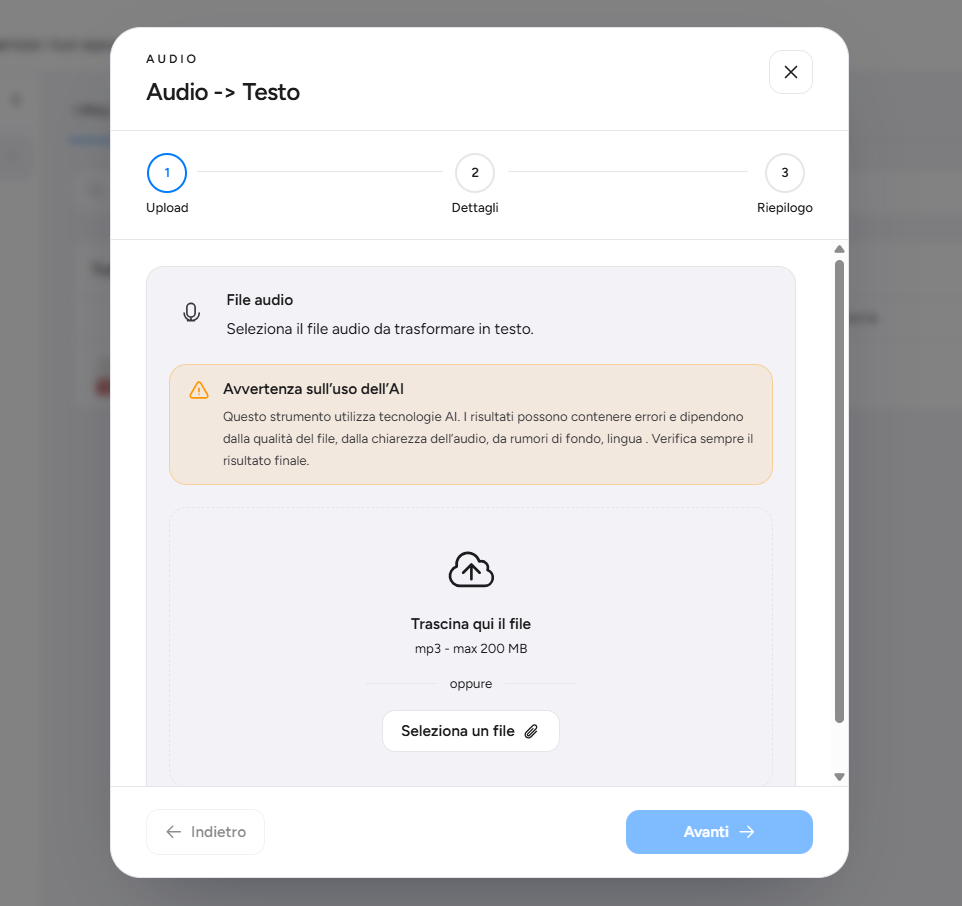
\includegraphics[width=\textwidth]{figures/fig-riprogettazione-fisica/strumenti-ai/ai_1.png}
        \caption{}
        \label{fig:ai_1}
    \end{subfigure}
    \qquad
    \begin{subfigure}[b]{0.47\textwidth}
        \centering
        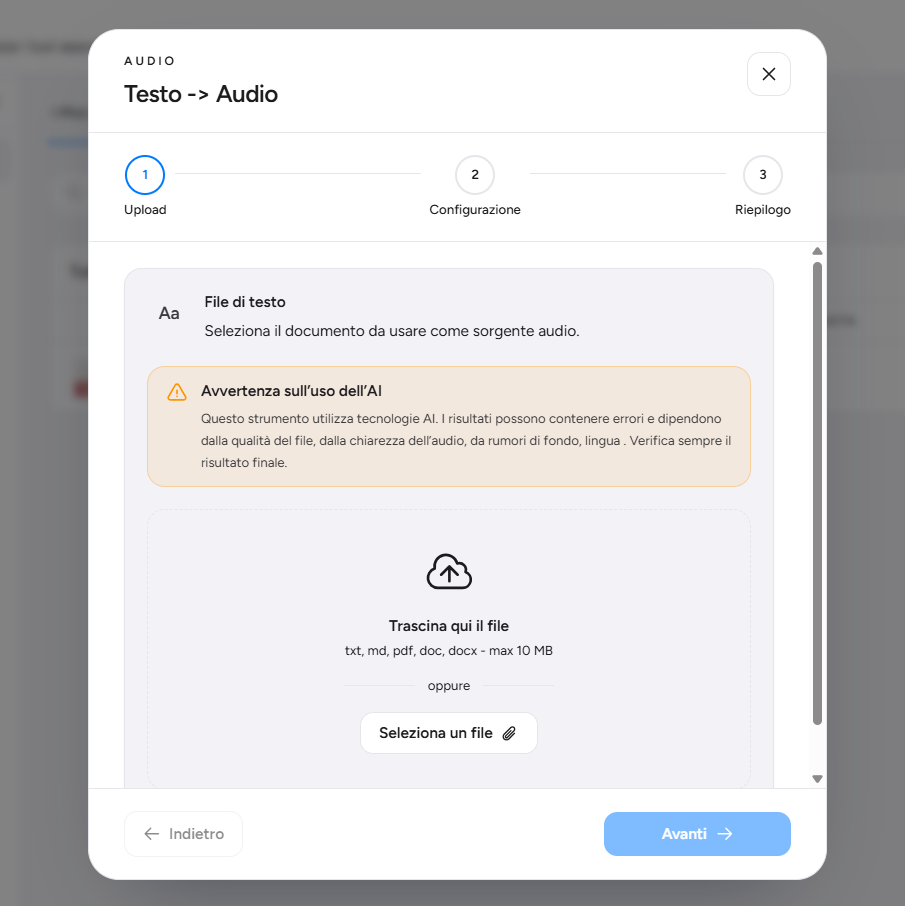
\includegraphics[width=\textwidth]{figures/fig-riprogettazione-fisica/strumenti-ai/ai_2.png}
        \caption{}
        \label{fig:ai_2}
    \end{subfigure}

    \caption{}
    \label{fig:steps1_ai}
\end{figure}

\item \textbf{Spinners and Loading Indicators} (Tidwell): Il pattern prevede di mostrare un'animazione o un indicatore dopo che l'utente ha avviato un'operazione e prima che ci sia una risposta, per comunicare che il sistema sta elaborando e prevenire che l'utente abbandoni il task o pensi che qualcosa sia andato storto. 
  È considerato obbligatorio quando un'operazione richiede più di un secondo, poiché oltre questa soglia l'utente tende a ritenere che l'interfaccia non stia funzionando. 
  Nella versione precedente lo strumento non forniva alcuna indicazione visiva sull'avanzamento della generazione, lasciando l'utente in attesa senza sapere se il sistema stesse effettivamente elaborando. Nella versione riprogettata, invece di un indicatore bloccante mostrato durante l'attesa, la lista file espone in modo persistente lo stato della generazione tramite etichette dinamiche, \textit{In coda}, \textit{In elaborazione}, \textit{Pronto} o \textit{Errore}, permettendo all'utente di monitorare l'avanzamento senza interrompere il proprio flusso di lavoro.

Problemi di usabilità risolti:
\begin{itemize}
  \item P50 (Feedback non chiaro sullo stato di avanzamento durante la generazione): Lo stato di elaborazione è ora sempre visibile nella lista file tramite etichette dinamiche che si aggiornano in tempo reale.
\end{itemize}

  \begin{figure}[H]
    \centering
    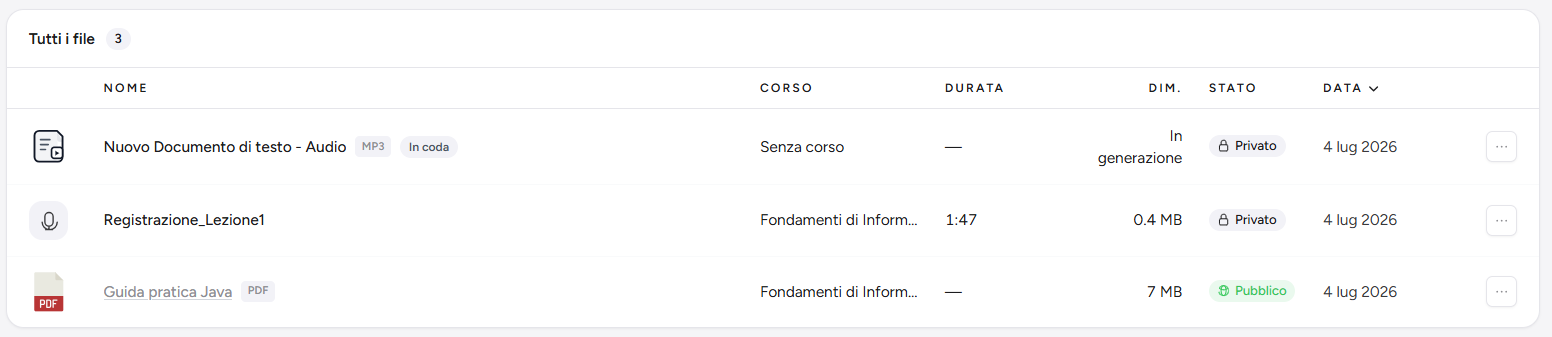
\includegraphics[width=0.8\textwidth]{figures/fig-riprogettazione-fisica/strumenti-ai/ai_4.png}
    \caption{}
    \label{fig:ai_4}
  \end{figure}

\end{itemize}

\paragraph{Altre modifiche}
La struttura delle funzionalità AI è stata radicalmente semplificata eliminando le pagine dedicate e integrando i generatori direttamente nella sezione \textit{Appunti}. \\

Problemi di usabilità risolti:
\begin{itemize}
  \item P41 e P44 (Icone microfono/cassa non funzionanti): Essendo ora le funzioni incorporate in un form di caricamento, le icone "falso bottone" nei titoli sono state rimosse.
  \item P42 (Posizionamento del bottone ”NUOVA TRASCRIZIONE”): Il comando è stato razionalizzato all'interno del flusso di creazione file in \textit{Appunti}. Stessa soluzione per il bottone "NUOVA AUDIO NOTE".

    \begin{figure}[H]
      \centering
      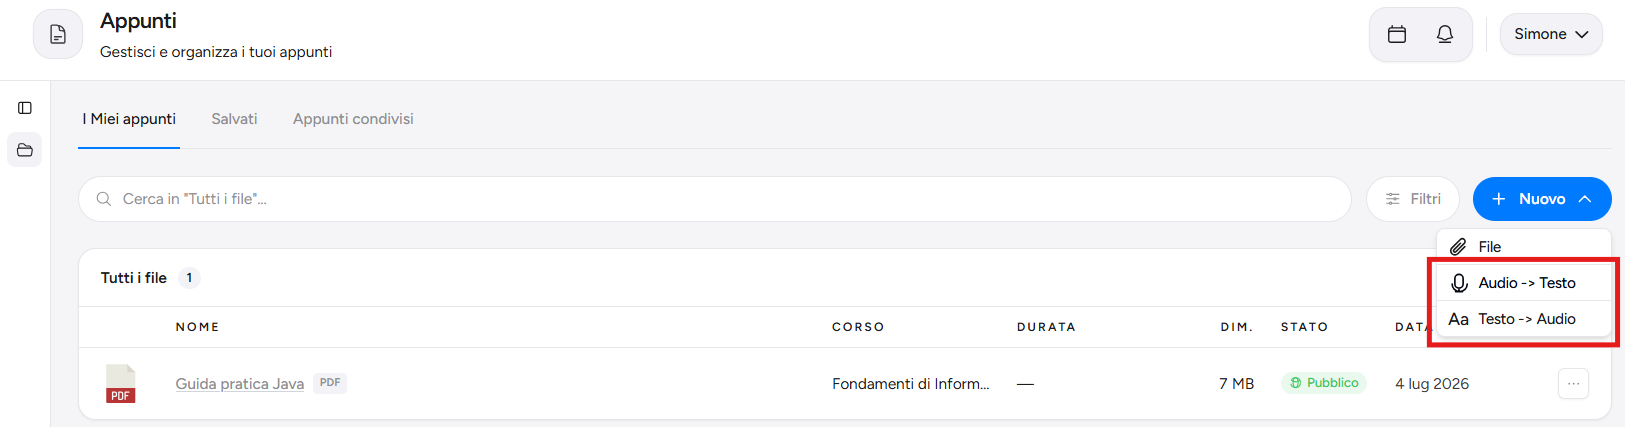
\includegraphics[width=0.8\textwidth]{figures/fig-riprogettazione-fisica/strumenti-ai/ai_3.png}
      \caption{}
      \label{fig:ai_3}
    \end{figure}

  \item P66 (Impossibilità di salvare o allegare): Entrambe le tipologie di file generati (audio e testo) possono ora essere salvate come nuovi appunti e allegate direttamente agli esami.
  \end{itemize}

  Generatore trascrizioni:
  \begin{itemize}
  \item P74 (Mancanza di struttura semantica): Il blocco di testo generato non è più uniforme, ma include ora i \textit{timestamp} per facilitare la consultazione e il riferimento all'audio originale.
\end{itemize}

Generatore audio:
\begin{itemize}
\item P45 (Incoerenza del tasto di conferma): Il pulsante è stato rinominato in \textit{Avvia}, garantendo coerenza terminologica.
\item P67 (Mancanza di supporto iconografico): Gli audio generati sono ora identificati da un'icona specifica nella lista file, permettendo di distinguerli a colpo d'occhio da PDF o altri documenti. Stessa soluzione anche per le trascrizioni.
\end{itemize}

\paragraph{Implementazioni aggiuntive}
La pagina di visualizzazione di una trascrizione è stata completamente riprogettata rispetto alla versione originale, che presentava il testo generato come un unico blocco non strutturato e privo di qualsiasi funzionalità aggiuntiva. Nella versione riprogettata la trascrizione è organizzata in segmenti, ciascuno accompagnato dal relativo intervallo temporale: cliccando su un segmento, il player audio posizionato in fondo alla pagina si sincronizza automaticamente al punto corrispondente dell'audio, permettendo all'utente di navigare rapidamente tra le parti della registrazione. Il contenuto è inoltre suddiviso in due tab, \textit{Trascrizione} e \textit{Riassunto}, così da offrire sia il testo completo sia una versione sintetica del contenuto senza dover scorrere l'intera pagina. In alto è presente un pulsante per scaricare la trascrizione in formato \texttt{.txt}, mentre il pannello laterale destro raccoglie i metadati del file (nome, durata, numero di segmenti, corso e data di caricamento) e un suggerimento contestuale nella parte inferiore. (Figura \ref{fig:ai_5})

  \begin{figure}[H]
    \centering
    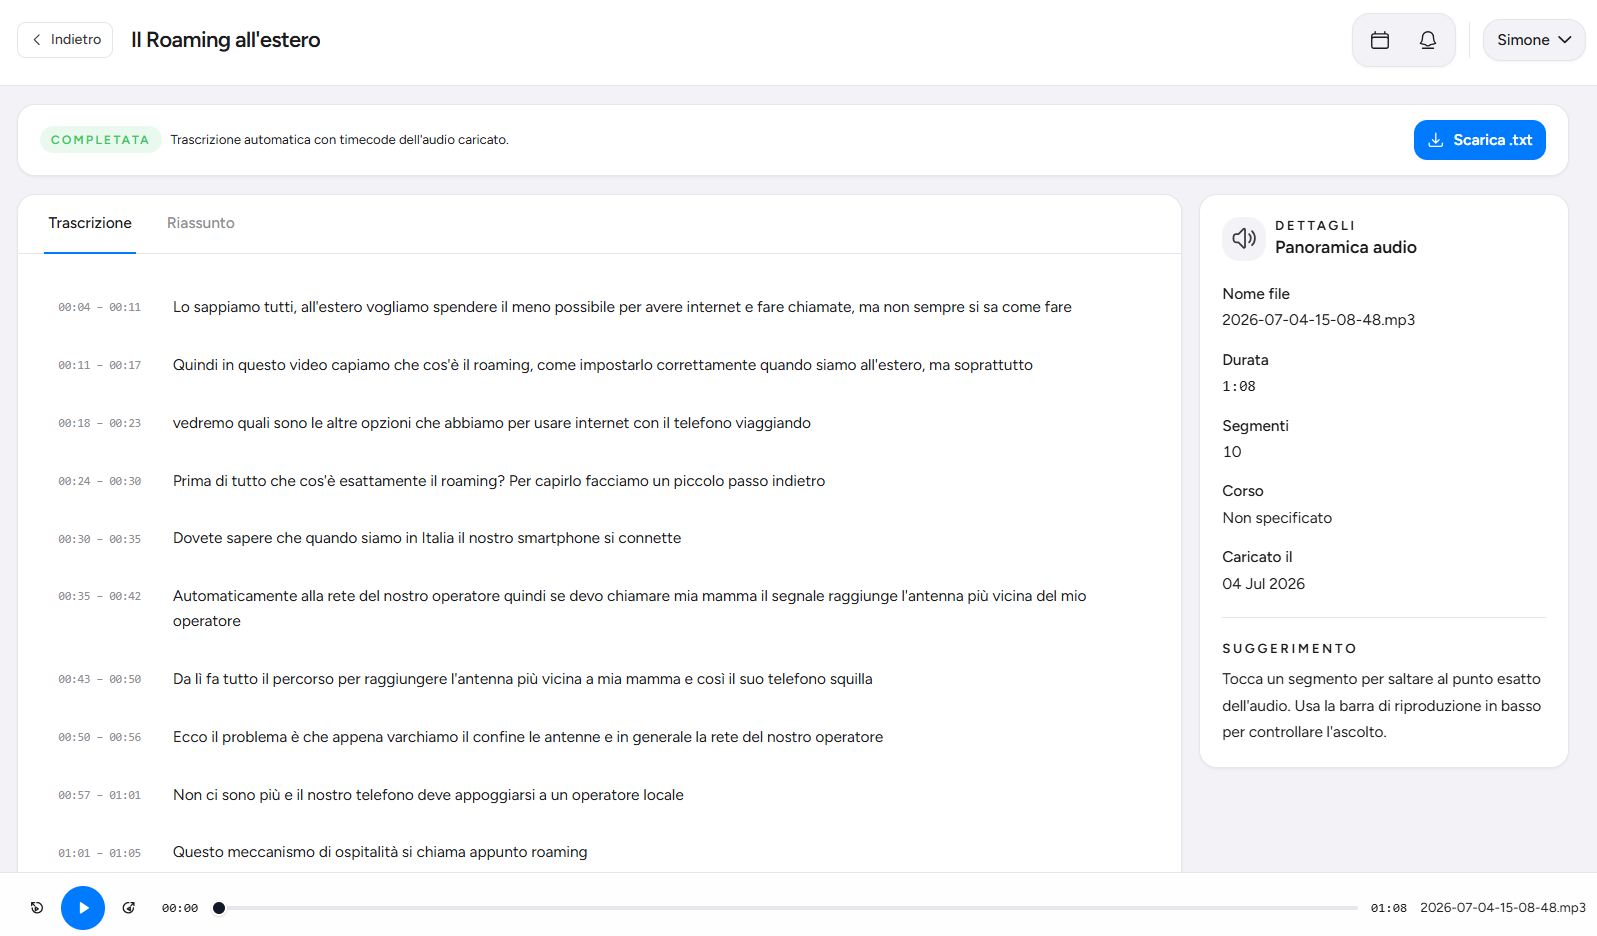
\includegraphics[width=0.8\textwidth]{figures/fig-riprogettazione-fisica/strumenti-ai/ai_5.png}
    \caption{}
    \label{fig:ai_5}
  \end{figure}

Per mantenere coerenza con la pagina di visualizzazione delle trascrizioni, anche la pagina di visualizzazione delle audio note è stata riprogettata adottando la stessa struttura: pulsante per scaricare il file MP3, player audio integrato per riprodurre direttamente il contenuto generato e pannello laterale destro con i metadati del file (nome, data di creazione, durata, tipo, dimensione, formato e voce utilizzata per la sintesi). (Figura \ref{fig:ai_6})

  \begin{figure}[H]
    \centering
    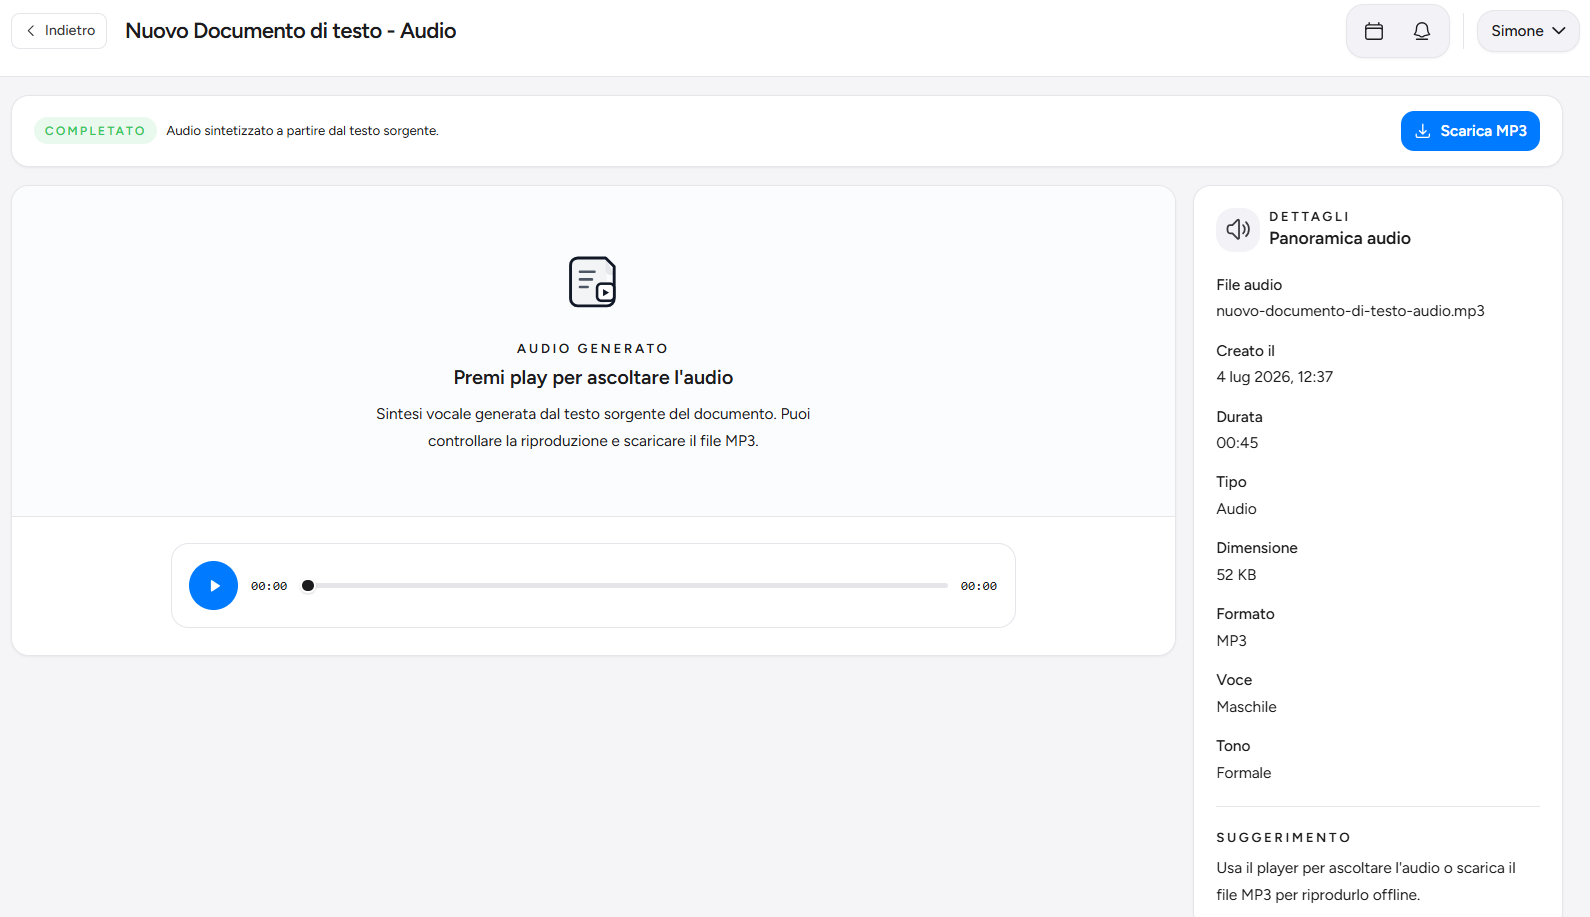
\includegraphics[width=0.8\textwidth]{figures/fig-riprogettazione-fisica/strumenti-ai/ai_6.png}
    \caption{}
    \label{fig:ai_6}
  \end{figure}